\chapter{Evaluation}

\label{Chapter4}

\lhead{Chapter 4. \emph{Evaluation}}

This chapter will evaluate a prototype implementation of the approach presented in chapter~\ref{Chapter3}.

The chapter starts with introducing the main goal and the experimental setup in sections~\ref{eval:sec:prerequisites} and~\ref{eval:sec:experimental_setup},
before evaluating the actual results in sections~\ref{eval:sec:ab_testing_features},~\ref{eval:sec:clustering}, and~\ref{eval:sec:adapting_the_application}.
% We round up this evaluation chapter with a summary and discussion, in sections~\ref{eval:sec:summary} and~\ref{eval:sec:discussion}.

\section{Prerequisites} % (fold)
\label{eval:sec:prerequisites}

For any of this user adaptation to have any actual use, we will need to find out whether there actually exists significant variation in feature adoption between clusters; it matters little whether users exhibit differing behavior with regard to existing functionality, unless this behavior yields a basis for predicting future behavior. We need an inductive bias.

As described in chapter~\ref{Chapter3}, a way of discovering whether this inductive bias is present in the user base is to investigate whether there is significant variance across the clusters in their members' adoption of new features. Thus, this question of whether the predictive bias exists will be included as a central part of the actual experiment itself, and be thoroughly discussed through the next sections.

Moreover, an arguably obvious, but imperative aspect of the proposed approach is that the users for whom adaptations are predicted must be identifiable over an extended amount of time. They must be present with the same cookie identifier both prior to clustering and after applying the adaptations.

\section{Experimental setup} % (fold)
\label{eval:sec:experimental_setup}

In the main experiment, we want to correlate the A/B test results with the user clusters, and see if variations are present. This rather simple scheme is illustrated in figure~\ref{fig:experimental-setup}.

\begin{figure}[h]
  \centering
    \includegraphics[width=0.5\textwidth]{Figures/experimental-setup}
    \caption{The experiment setup. The output of the correlation component (in gray) will determine the outcome of the experiment.}
    \label{fig:experimental-setup}
\end{figure}

The main hypothesis is:

\begin{quote}
  Different variations of a service may perform differently among ``different kinds of users''. These variations can be used as inductive bias on which general user adaptations can be based.
\end{quote}

Two sources of input will serve as input data to test the hypothesis:

\begin{enumerate}
  \item A/B test results
  \item User clusters
\end{enumerate}

The data from the A/B test results describe each person's designated variant, and the resulting performance. See table~\ref{tab:person_variants} for some example data.

\begin{table}[h]
  \centering
  \begin{tabular}{|l|l|ll|}
    \hline
    Person & Variant & Entered room & Entered conversation \\ \hline
    p1     & A       & no           & no  \\
    p2     & A       & yes          & yes \\
    p3     & B       & yes          & no  \\
    p4     & A       & no           & no  \\
    p5     & B       & yes          & yes \\ \hline
  \end{tabular}
  \caption{Each person has one assigned variant, and some performance measures.}
  \label{tab:person_variants}
\end{table}

The user cluster data contain the same persons as the test results in table~\ref{tab:person_variants} and the clusters they have been assigned to, as illustrated in table~\ref{tab:person_clusters}.

\begin{table}[h]
  \centering
  \begin{tabular}{|l|l|}
    \hline
    Person & Cluster \\ \hline
    p1     & 1 \\
    p2     & 2 \\
    p3     & 1 \\
    p4     & 1 \\
    p5     & 2 \\ \hline
  \end{tabular}
  \caption{Persons have been assigned to to clusters.}
  \label{tab:person_clusters}
\end{table}

These data sources are aggregated with regard to variant and cluster, and the relative success rates compared.

The next sections walk through and evaluate the actual results in the context of the experiment described in this section.

\subsection{Evaluation case: New appear.in landing page}
\label{eval:sub:new_landing_page}

\begin{figure}[h]
  \centering
    \begin{subfigure}[t]{0.8\textwidth}
      \centering
      \includegraphics[width=\textwidth]{Figures/screenshots/ab-frontpage/variation-off}
      \caption{Variation $A$.}
      \label{fig:variation_a}
    \end{subfigure}

    \vspace{1em}

    \begin{subfigure}[t]{0.8\textwidth}
      \centering
      \includegraphics[width=\textwidth]{Figures/screenshots/ab-frontpage/variation-on}
      \caption{Variation $B$.}
      \label{fig:variation_b}
    \end{subfigure}

  \caption{Variations in the new landing page experiment.}
  \label{fig:variations}
\end{figure}

To test the hypothesis, we performed a controlled experiment on the user base of appear.in as we rolled out a new landing page.

The experiment stood between the old landing page, the control treatment, and a new design. We shall from here on refer to them as variation $A$ and $B$, respectively. The two competing variations are depicted in figure~\ref{fig:variations}.

\section{A/B testing feature variations}
\label{eval:sec:ab_testing_features}

After running through the test period with an even randomized user split between the two variations, the results were in. In total, just over 20,000 people were included in the experiment and were served one of the two variations.

The two were compared head to head for two different performance metrics:

\begin{description}
  \item[Visited room] \hfill \\
    The number of users going from the landing page and into a room.
  \item[In a conversation] \hfill \\
    The number of users going from the landing page and into a conversation. This entails that the person in question has understood the concept of how one establishes a conversation, which can be seen as the next step of user activation after entering a room.
\end{description}

The aggregate numbers are shown in tables~\ref{tab:performance_room} and~\ref{tab:performance_conversation}.

\begin{table}[h]
  \begin{tabular}{|l|r|r|r|r|r|}
    \hline
    Variation & People & Conversions & Average conversion & Improvement & Certainty \\ \hline
    $A$       & 10,100 & 7,946       & 78.67\%            & -           & -         \\ \hline
    $B$       &  9,931 & 7,883       & 79.38\%            & 0.90\%      & 89.04\%   \\ \hline
  \end{tabular}
  \caption{Comparison of ``Visited room'' conversion ratios for variations $A$ and~$B$.}
  \label{tab:performance_room}
\end{table}

\begin{table}[h]
  \begin{tabular}{|l|r|r|r|r|r|}
    \hline
    Variation & People & Conversions & Average conversion & Improvement & Certainty \\ \hline
    $A$       & 10,009 & 3,602       & 35.99\%            & -           & -         \\ \hline
    $B$       & 10,172 & 3,781       & 37.17\%            & -3.29\%     & 95.98\%   \\ \hline
  \end{tabular}
  \caption{Comparison of ``In a conversation'' conversion ratios for variations $A$ and~$B$.}
  \label{tab:performance_conversation}
\end{table}

Figures~\ref{fig:performance_room} and~\ref{fig:performance_conversation} show how the variations performed with respect to the two metrics, both with variation $B$ plotted relative to variation $A$ as the baseline.

\begin{figure}[h]
  \centering
  \begin{subfigure}[t]{0.8\textwidth}
    \includegraphics[width=\textwidth]{Figures/plots/ab-frontpage/room-conversions-plot-only}
    \caption{Comparison of the variations by the ``Visited room'' metric.}
    \label{fig:performance_room}
  \end{subfigure}

  \vspace{1em}

  \begin{subfigure}[t]{0.8\textwidth}
    \includegraphics[width=\textwidth]{Figures/plots/ab-frontpage/conversation-conversions-plot-only}
    \caption{Comparison of the variations by the ``In a conversation'' metric.}
    \label{fig:performance_conversation}
  \end{subfigure}

  \caption{Variation $B$ performance, relative to variation $A$ (the baseline).}
  \label{fig:ab_performance_plots}
\end{figure}

As we can plainly see, variation $B$ performs slightly better at moving people into rooms, but evidently fails to communicate the conversation concept, leading to a relative decrease in actual subsequent conversations.

While these numbers and plots set the scene, they are not very interesting from our adaptation perspective. We are first and foremost interested in seeing whether these numbers vary significantly between segments of the user base, thus providing us with a predictive bias from which we can extrapolate our user adaptations.

Section~\ref{eval:sec:adapting_the_application} breaks the numbers down cluster by cluster, and investigates to what degree this information can be used to power user adaptations.

\section{User clustering} % (fold)
\label{eval:sec:clustering}

\begin{figure}[h]
  \centering
    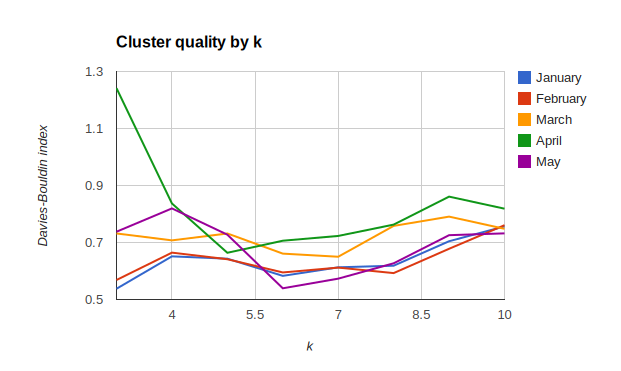
\includegraphics[width=\textwidth]{Figures/plots/k-vs-db/jan-may}
    \caption{$k$ vs. Davies-Bouldin index, for clusters with data for January to May.}
    \label{fig:k_vs_db}
\end{figure}

Figure~\ref{fig:k_vs_db} shows a set of clustering runs. Data was timeboxed per month, from January thru May, and k-means was run for a range of $k$ from 3 up to 10. The other parameters used, as well as the particular resulting cluster set from February, are discussed in further detail in section~\ref{eval:sec:clustering_results}.

\subsection{Varying demographics}
\label{eval:sub:varying_demographics}

Through the spring of 2014, appear.in received quite a bit of media attention, and different times saw user influx from a large variety of demographic origins.

The coverage varied from technical showcases and industry newsletters to the service being featured in Hungarian newspapers and on BBC World News. Moreover, these spurs of media attention seems to mostly have been independently initiated, and as a result we saw large peaks of visitors from quite specific locations at different times. Overall, though, the traffic was distributed quite evenly over a large number of geographical areas.

The \emph{timespan} parameter was used extensively to compare these, and aided in avoiding becoming subject to these various demographical biases.

\subsection{Initial clustering results}
\label{eval:sec:clustering_results}

The data used in this analysis stems from February 2014.

The clustering results shown in this section were produced by choosing the best of 5 k-means runs, ``best'' being defined by their Davies-Bouldin indices (see section~\ref{survey:evaluating_clusters} for a brief description of this evaluation metric). This process was performed for $k$ parameter values from 3 to 10, where $k = 8$ yielded the best result.

Although mostly irrelevant to the experiment, a detailed analysis of the clusters depicted in figure~\ref{fig:radar-clusters-february} is available in~\ref{appendix:clustering_results}.

Data from January and March yield more or less the same results, although they are a bit less clear. This could be due to media events and holidays generating more skewed data than usual.

\begin{figure}[h]
  \centering
    \includegraphics[width=0.8\textwidth]{Figures/clusterings/confluence-post/comp-02-feb}
    \caption{Radar chart comparing clusters generated from data for February 2014.}
    \label{fig:radar-clusters-february}
\end{figure}

The radar chart in figure~\ref{fig:radar-clusters-february} shows the centroids of 6 large clusters $C$ relative to each other.

Each dimension's centroid values $\mu_i \in \mu$ have been scaled by a factor of $\frac{10}{\max_{c \in C}{c_i}}$, to fit nicely inside the chart.

The features used in this particular clustering run are (clockwise around the chart):

\begin{enumerate}
  \item chat messages sent
  \item conversations (2+ persons present in room)
  \item rooms claimed
  \item rooms followed
  \item unique rooms used
  \item conversation network size (ie. number of unique other users within 2 degrees of conversation separation)
\end{enumerate}

Most of these features are quantified by counting the number of relevant events logged for each user.

% \subsection{The applicability of manual cluster analysis}
% \label{eval:sub:cluster_analysis_applicability}
%
% When analyzing a set of clusters, it is tempting to focus on the extremes -- the easily stereotyped user profiles -- as we have done above. However, we see that a vast majority of users are indeed too close to the origo to be confidently labelled as some kind of stereotype.
%
% Thus, although tempting from a business intelligence type of perspective, manual cluster stereotyping becomes a highly speculative exercise whose conclusions are extremely hard to confirm without demographic data readily available.
%
% We will return to this issue in chapter~\ref{Chapter5}.

\section{Adapting the application} % (fold)
\label{eval:sec:adapting_the_application}

The task of adapting the application brings together previous A/B test results and the clusters discovered, as described in sections~\ref{eval:sec:ab_testing_features} and~\ref{eval:sec:clustering}.

\begin{table}[h]
  \centering
  \begin{tabular}{| l |  rrr| rrr| rrr| c|}
\hline
 Variations & \multicolumn{3}{|c|}{off} & \multicolumn{3}{|c|}{on} & \multicolumn{3}{|c|}{total} & \\
\hline
 Clusters & n & c & \% & n & c & \% & n & c & \% & preferred \\
\hline
Cluster 2135 & 42 & 0 & 0.00 & 43 & 0 & 0.00 & 85 & 0 & 0.00 & off \\
Cluster 2136 & 21 & 9 & 42.86 & 16 & 11 & 68.75 & 37 & 20 & 54.05 & on \\
Cluster 2137 & 156 & 75 & 48.08 & 152 & 67 & 44.08 & 308 & 142 & 46.10 & off \\
Cluster 2138 & 151 & 90 & 59.60 & 160 & 113 & 70.62 & 311 & 203 & 65.27 & on \\
Cluster 2139 & 118 & 106 & 89.83 & 133 & 125 & 93.98 & 251 & 231 & 92.03 & on \\
Cluster 2140 & 180 & 145 & 80.56 & 165 & 134 & 81.21 & 345 & 279 & 80.87 & on \\
\hline
\end{tabular}

  \caption{Success of the different variations for each cluster $C$.}
  \label{tab:variation_cluster_correlations}
\end{table}

Table~\ref{tab:variation_cluster_correlations} shows the success of the different variations for each cluster. We see that there are indeed clear differences between them, and can therefore reasonably state that there exists an inductive bias on which predictions about future behavior can be based.

However, let us not jump to conclusions. In~\ref{eval:sec:ab_testing_features} we ran a controlled experiment with just over 20,000 people, and here we are seeing numbers totaling at just over 1300.

To illustrate the point of the next section, the clusters in table~\ref{tab:variation_cluster_correlations} were identified based on data from just \emph{before} the A/B experiment was run. As we can plainly see, the majority of the clustered users did not return to the service within the experiment time period, resulting in an extremely low participation rate.

\section{Identity persistence}
\label{eval:sec:identity_persistence}

The numbers in~\ref{eval:sec:adapting_the_application} tells us that it may not be enough to be able to predict what the current user base wants. What we \emph{really} want is to use this information to improve the service for returning users. However, it is not enough to have predictive bias if we're unable to recognize our returning users. This section analyzes the impact of cookie impermanence.

As has been discussed extensively already, a major difficulty in adapting applications such as appear.in to its users is that there is no concrete notion of a user. Users are anonymous, and the only way they are being tracked at all is through a random hash set in a tracking cookie (see section~\ref{survey:client_side_identity}). How exactly, though, does this affect our adaptation efforts?

One way of gauging this is to look at the number of users we see returning. As an extreme, consider a user who does not keep cookies across sessions. Every time this user returns to the site, he will be treated as a new, previously unseen user. By extension, for how long do we see each tracking cookie return before we never see it again?

Table~\ref{tab:returning_users} shows the decline over time of the number of returning users, as compared to the user base of January, February and March.

\begin{table}[h]
  \centering
  \begin{tabular}{|l|rrrrr|}
    \hline
    Users from month & 1 month & 2 months & 3 months & 4 months & 5 months \\ \hline
    January          & 23.20\% & 5.10\%   & 2.90\%   & 1.90\%   & 0.90\%   \\
    February         & 20.20\% & 3.80\%   & 2.10\%   & 1.10\%   & -        \\
    March            & 23.20\% & 5.40\%   & 2.90\%   & -        & -        \\ \hline
  \end{tabular}
  \caption{The degree to which a monthly unique set of users are seen again after $n$ months.}
  \label{tab:returning_users}
\end{table}

Two plots of these numbers can be seen in figure~\ref{fig:perceived_user_persistence}, with normal scale and logarithmic scale.

As we see, just over 20\% are seen again the month after they first visit the site. Only about 20\% of these users again make it through to the subsequent month. After three months, less than 3\% remain in all three cases.

As a more general measure of this, take figure~\ref{fig:user_timediffs}. The histogram shows the number of persons having visited the site at least twice, placed in bins reflecting the number of days separating their first and last recorded visit. As we see, on average it takes less than a month before the number of users has fallen an entire order of magnitude.

\begin{figure}[t]
  \centering
  \begin{subfigure}[t]{0.9\textwidth}
    \includegraphics[width=\textwidth]{Figures/plots/timediffs/timediffs}
    \caption{Linear scale.}
  \end{subfigure}

  \begin{subfigure}[t]{0.9\textwidth}
    \includegraphics[width=\textwidth]{Figures/plots/timediffs/timediffs-log}
    \caption{Logarithmic scale.}
  \end{subfigure}

  \caption{Returning users' site usage time spans.}
  \label{fig:user_timediffs}
\end{figure}

\subsection{User retention factors}
\label{eval:retention_factors}

The perceived rate of retention is subject to three different factors:

\begin{enumerate}
  \item The user did not use the service again.
  \item The user cleared the browser cookies.
  \item The user changed browser or computer.
\end{enumerate}

There is all reason to believe that we are looking at a combination between all three, yet hard to know how much each contributes to the trend. We naturally assume that most users perceived as not returning simply do not return.

However, the survey performed by Teltzrow and Kobsa~\cite{Teltzrow2004}, as discussed in section~\ref{survey:privacy_vs_personalization}, states that more than half of all users clear their cookies periodically, and a significant amount of users reject cookies altogether. We will therefore assume that the last two factors also contribute in a significant degree to these numbers.

\begin{figure}[t]
  \centering
  \begin{subfigure}[t]{\textwidth}
    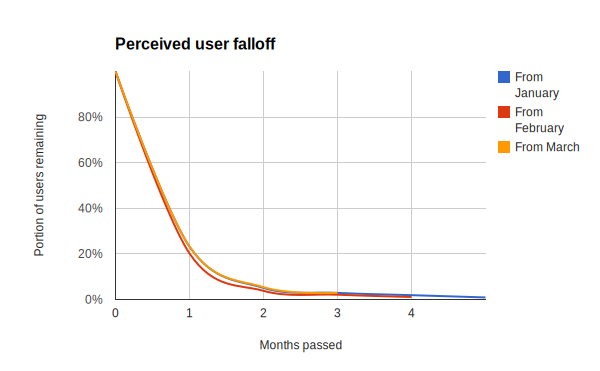
\includegraphics[width=\textwidth]{Figures/plots/user-dropoff/months-jan-mar}
    \caption{Perceived user persistence.}
  \end{subfigure}

  \vspace{1em}

  \begin{subfigure}[t]{\textwidth}
    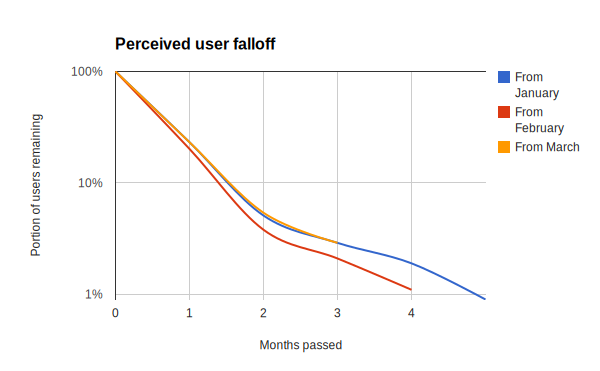
\includegraphics[width=\textwidth]{Figures/plots/user-dropoff/months-jan-mar-log}
    \caption{Perceived user persistence, logarithmic scale.}
  \end{subfigure}

  \caption{Perceived user persistence, illustrating the identified user dropoff rate.}
  \label{fig:perceived_user_persistence}
\end{figure}
